\section{Graphical User Interface}
\label{sec:gui}
%
Our graphical user interface (GUI) is quite costly in terms of
computation. So we emphatically recommend that you {\bf properly
configure the hardware acceleration of your graphics card}.
If you still have performance
issues make the window as small as possible. The smaller
the window is the less is the processing cost.

The SSR GUI tries to enable samplebuffer support to enable
anti-aliasing of the screen output. It will tell you if it didn't
work out. Check Fig.~\ref{fig:anti_aliasing} to get an idea of
the influence of anti-aliasing.
%
One day we will also implement a variable frequency for the
screen update so that you can slow it down if CPU load is too high. Of course it
won't look as nice then.

\begin{figure}[htbp]
\begin{center}
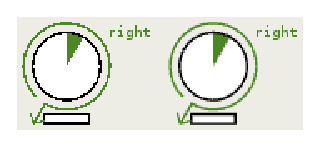
\includegraphics[scale=1]{anti_aliasing}
\caption{\label{fig:anti_aliasing}{No anti-aliasing on the left image.}}
\end{center}
\end{figure}

\begin{figure}[!t]% place the figure on top of the page
\begin{center}
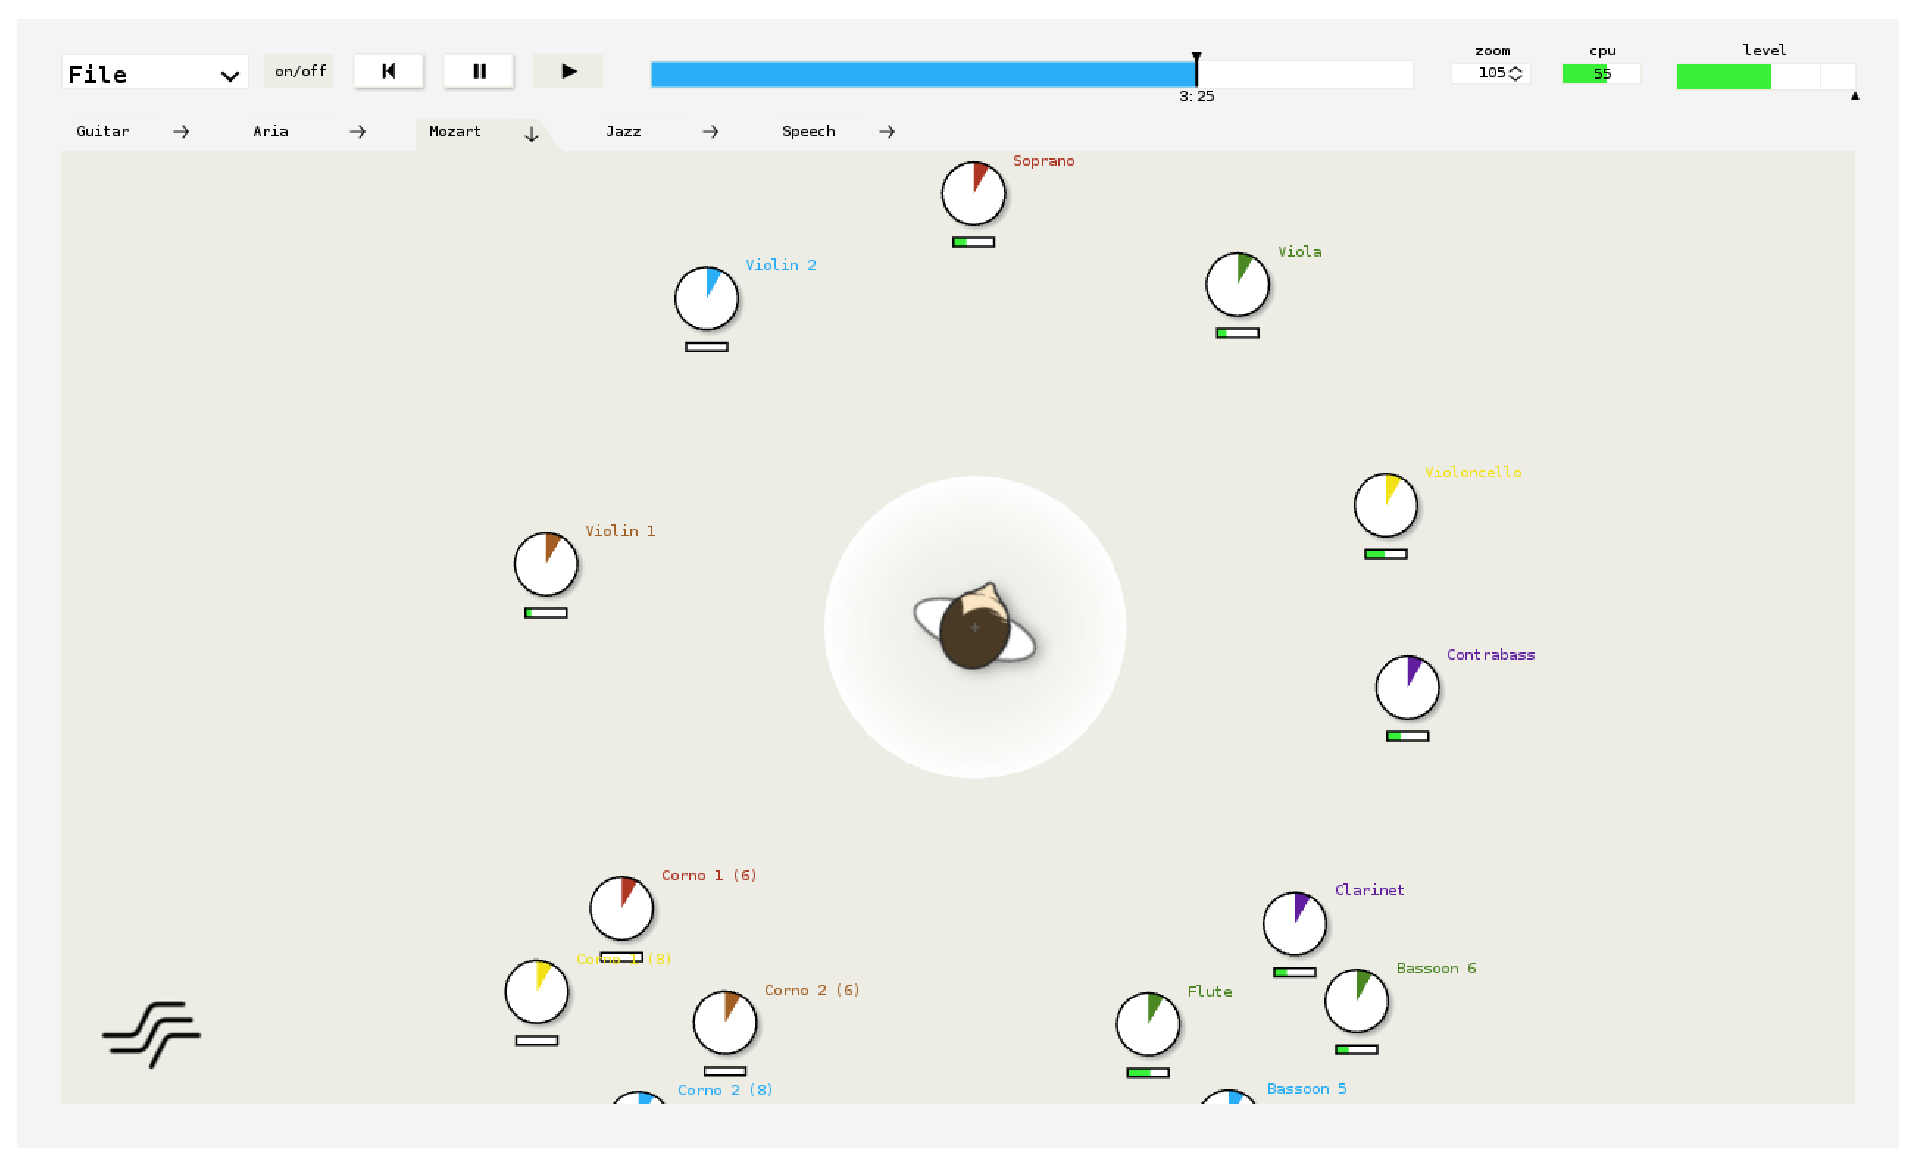
\includegraphics[width=\linewidth]{screenshot}
\caption{\label{fig:screenshot}{Screen shot of the SSR GUI.
%The current
%loudspeaker setup is a ring of 56 loudspeakers plus a subwoofer. In this case,
%WFS rendering was chosen. Both ``Ambiance'' sources emit plane waves, all
%other sources are point sources. Source ``Vocals'' is selected and the corresponding
%loudspeaker activity is indicated. Source ``Bass guitar'' is static and source
%``Guitar \& Keys'' is muted.
}}
\end{center}
\end{figure}
%
\subsection{General Layout}

The graphical user interface (GUI) consists mainly of an
illustration of the scene that you are hearing and some interaction
tools. The renderer type is indicated in the window title.
See a screen shot in Fig.~\ref{fig:screenshot}.

On the top left you will find the file menu where you can open files, save
scenes, and quit the application. So far only the \emph{save scene as\dots}
option is available. That means every time to save the current scene you will
be asked to specify the file name. This will be made more convenient in the
future.

Next to the file menu, there is a button which lets you activate and deactivate
the audio processing. Deactivating the audio processing does not necessarily
lower the CPU load. It means rather that the SSR won't give any audio output,
neither for involved audio files nor for live inputs.

Next to the processing button, you find the transport section with buttons to
skip back to the beginning of a scene, pause replaying, and continue/start
playing. Note that pausing a scene does not prevent live inputs from being
processed. To prevent audio output switch off processing (see above). You may
also replay while processing is switched off to navigate to a certain point in
time in the respective scene.

In the top middle section of the GUI there is the audio scene time line.
By default, it shows a time interval of two minutes duration. Whenever
the progress exceeds the displayed time interval the latter is shifted
such that the progress is always properly indicated.
Below the handle, there is a numerical
indication of the elapsed time with respect to the beginning of the scene.
See Sec.~\ref{sec:mouse_actions}
for information on how to operate on the time line.

To the right of the time line there's the CPU load gauge. It
displays the average CPU load as estimated by the JACK audio
server on a block-wise basis.
Further right there's the label to indicate the current zoom factor
in percent.

And finally, on the top right you find the master level meter combined with the
master volume fader. The colored bar indicates an estimation of the relative
maximum audio level in dB, also updated block-wise. The left boundary of the
meter is at -50~dB; the right boundary is at +12~dB. The black triangle below
the colored bar indicates the master volume in dB. Click somewhere into the
widget and the master volume gets additionally displayed as a number. Note that
this meter displays full scale, i.e.~above 0~dB clipping and thus distortion of
the output signal occurs! 0~dB is indicated by a thin vertical line.

In the row below the transport section, you occasionally find some tabs giving
fast access to a number of scenes. These tabs can be defined in a file. By 
default, the file \texttt{scene\_menu.conf} in the current working directory is
assumed; there is also an option to specify the file name in the SSR 
configuration file. Refer to Sec.~\ref{sec:ssr_configuration_file}. The 
configuration file for the tabs may contain something like the following:
%
\begin{verbatim}
# This file configures the menu for the scene selection.
#
scenes/dual_mono.asd Guitar######### comments are possible
scenes/jazz.asd Jazz
scenes/rock.asd Rock
#scenes/speech.asd Speech
scenes/live_conference.xml live conference
\end{verbatim}
%
The syntax is as follows:
\begin{itemize}
\item[-] Everything after a hash symbol (\#) in a line is ignored.
\item[-] A valid entry consists of the path (relative or absolute)
to ASDF file (or pure audio file) followed by space and a short
keyword that will be displayed on the respective tab on the screen.
\end{itemize}
%
Of course, also audio files can be specified instead of \texttt{.asd}s. Note
that so far, no syntax validation is performed, so watch your typing. We
furthermore recommend that you keep the keywords short because space on the
screen is limited. Note also that only those tabs are displayed which fit on
the screen.

The SSR always tries to find the file \texttt{scene\_menu.conf} in its current
working directory (or at the location specified in the SSR configuration file). 
If is does not find it no tabs will be displayed in the GUI.
So you can have several of such files at different locations. We have added an
example in folder \texttt{data/}.

The main part of the screen is occupied by the graphical
illustration of the scene that you are hearing. The orientation of the coordinate
system is exactly like depicted in Fig.~\ref{fig:coordinate_system}.
I.e., the $x$-axis points to the right of the screen, the $y$-axis points to the top
of the screen. The origin of the coordinate system is marked by a cross, the reference
is marked by a rhomb. The direction ``straight in front'' is typically assumed to be
vertically upwards on the screen, especially for binaural techniques. We do so as well.
Note that in this case ``straight in front'' means $\alpha = 90^\circ$ and NOT
$\alpha=0^\circ$.

In Fig.~\ref{fig:screenshot} you see a number of sound sources with their
individual audio level meters (combined with their individual volume
sliders) underneath. The left hand boundary of the level meter is at -50~dB; the right
hand boundary is at 0~dB. Spherical sources don't have any additional
decoration. The wave front and propagation direction of plane waves
are indicated.

You also see icons for the loudspeakers of the current rendering
setup (if the currently applied technique employs any).
%In 
%Fig.~\ref{fig:screenshot} you see the system that is installed in our
%Usability laboratory. It is a ring of a diameter of a bad 3
%meters hosting 56 equiangularly spaced loudspeakers plus a subwoofer.
%
%The rhombus inside the loudspeaker ring
%indicates the location and orientation of the reference point of the
%current setup.

\subsection{Mouse Actions}
\label{sec:mouse_actions}

The GUI is designed such that the most important functionalities
can be accessed via a touch screen. Thus, it mostly employs 'left
clicks' with the mouse.

The use of the file and transport section is rather intuitive so we
won't further explain it here. The time line can be used to jump to
a certain position within the sound scene and it also shows the
progress of the scene. Click into the white/blue area of the time
line in order to jump to a specific point in time, or drag the
handle to fast forward or rewind. Left-clicking to the right of the
time line skips forward by 5 seconds, left-clicking to the left of
the time line skips back by 5 seconds. Double-clicking on the time
line skips back to the beginning of the scene. Right-clicking on the
time line opens an input window in order that you can numerically
specify the time instant to jump to (refer to
Sec.~\ref{sec:keyboard_actions}).

You can change the zoom either by clicking into the zoom label and
dragging up or down for zooming in or out. Alternatively, you can use the
mouse wheel.
Clicking and dragging on the background of the screen lets you move
inside the scene. A double-click brings you back to the default
position and also defaults the zoom.

Clicking and dragging on a sound source lets you select and move it. Note that
you cannot directly manipulate the propagation direction of plane waves. It's
rather such that plane sources always face the reference point. To change their
direction of incidence move the plane wave's origin point to the appropriate 
position. Right clicking on a sound source opens a window which lists the 
properties of the source such as position, volume, etc. Refer to 
Fig.~\ref{fig:screenshot_spd} and Sec.~\ref{sec:source_properties_dialog}.

A right mouse click on the scene background lets you select multiple
sound sources via a rubber band.

If you hold the \texttt{Ctrl} key pressed during any mouse action then you
operate on all selected sound sources at the same time (i.e.~mute,
move, etc.~them).

Click on the SSR logo and you'll see the \emph{About the SSR}
information.

\subsubsection{Source Properties Dialog}
\label{sec:source_properties_dialog}

\begin{figure}
\begin{center}
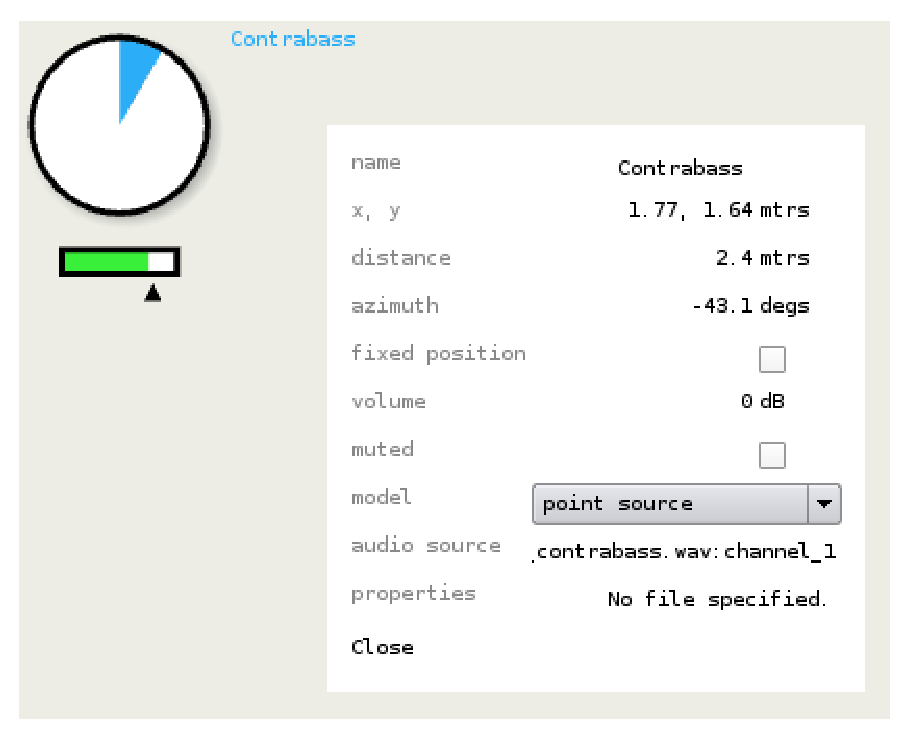
\includegraphics[scale=0.4]{screenshot_spd}
\caption{\label{fig:screenshot_spd}{Source properties dialog}}
\end{center}
\end{figure}

The source properties dialog can be accessed via a right click on a source and 
shows information about the actual state of the selected source. Its main 
purpose is to provide the possibility of an exact positioning of sources. The 
properties \texttt{fixed position}, \texttt{muted} and \texttt{model} can be 
changed. Please refer to figure \ref{fig:screenshot_spd} to see the complete 
list of properties this dialog shows. 

\subsection{Keyboard Actions}
\label{sec:keyboard_actions}
%
A number of keyboard actions have been implemented as listed below. Recall that also
some keyboard actions are available when the SSR is run without GUI (refer to 
Sec.~\ref{sec:running_ssr}).
%
\begin{itemize}
\item[] \texttt{+/-}: if no sound source is selected: raise/lower master volume by 1dB,\\
  otherwise raise/lower the selected sources' volume by 1dB
\item[] \texttt{Arrow up/down/left/right}: navigate in scene
\item[] \texttt{Space}: toggles the play/pause state
\item[] \texttt{Backspace}: skip to beginning of scene
\item[] \texttt{Return}: calibrate tracker (if present). When pressed, the instantaneous\\
  orientation is assumed to be straight forward (i.e.~90$^\circ$ azimuth)
\item[] \texttt{Ctrl}: when pressed, multiple sound sources can be
selected via mouse clicks or operations can be performed on multiple sources simultaniously
\item[] \texttt{Ctrl+Alt}: individual sound sources can be
deselected from a larger selection via a mouse click or the rubber band
\item[] \texttt{Ctrl+a}: select all sources
\item[] \texttt{f}: toggles the position-fix-state of all selected sound sources (sources
  which can not be moved are marked with a little cross)
\item[] \texttt{m}: toggles the mute state of all selected sound sources (muted sources
  are displayed with a grey frame instead of a black one)
\item[] \texttt{p}: toggles the source model between \emph{plane wave} and \emph{point source}
\item[] \texttt{s}: if no source selected: unsolos all potentially soloed sources,\\
  otherwise: solos selected sound sources.
\item[] \texttt{Ctrl+s}: opens the \emph{save scene as\dots} dialog
\item[] \texttt{F11}: toggles window fullscreen state
\item[] \texttt{1-9}: select source no.~1-9
\item[] \texttt{0}: deselect all sources
\item[] \texttt{Ctrl+c}: quit
\item[] \texttt{Ctrl+t}: open text edit for time line. The format is
\texttt{hours:mins(2digits):secs(2digits)} whereby \texttt{hours:}
and \texttt{hours:mins(2digits):} can be omitted if desired.
\item[] \texttt{Esc}: quit
\end{itemize}
%
%
%
